\documentclass{article}%
\usepackage[T1]{fontenc}%
\usepackage[utf8]{inputenc}%
\usepackage{lmodern}%
\usepackage{textcomp}%
\usepackage{lastpage}%
\usepackage{parskip}%
\usepackage[top=1.2in,bottom=1in,left=0.6in,right=0.6in,headsep=0.8in]{geometry}%
\usepackage{amsmath}%
\usepackage{graphicx}%
\usepackage{needspace}%
\usepackage{color}%
\usepackage{longtable}%
\usepackage{multirow}%
\usepackage[table]{xcolor}%
\usepackage{fancyhdr}%
\usepackage{tabularx}%
%
\definecolor{OsdagGreen}{HTML}{D5DF93}%
\fancypagestyle{header}{ 
\renewcommand{\headrulewidth}{0pt}%
\renewcommand{\footrulewidth}{0pt}%
\fancyhead{ 
}%
\fancyfoot{ 
}%
\fancyhead[C]{ 
\begin{tabularx}{\textwidth}{|l|p{6cm}|l|X|}%
\hline%
\rowcolor{OsdagGreen}%
Company Name&&Project Title&\\%
\hline%
\rowcolor{OsdagGreen}%
Group/Team Name&&Subtitle&\\%
\hline%
\rowcolor{OsdagGreen}%
Designer&&Job Number&\\%
\hline%
\rowcolor{OsdagGreen}%
Date&12 /05 /2020&Client&\\%
\hline%
\end{tabularx}
}%
\fancyfoot[R]{ 
Page \thepage\ of \pageref{LastPage}
}
}%
%
\begin{document}%
\normalsize%
\pagestyle{header}%
\section{Input Parameters}%
\label{sec:InputParameters}%
\renewcommand{\arraystretch}{1.2}%
\begin{longtable}{|p{5cm}|p{2cm}|p{2cm}|p{2cm}|p{5cm}|}%
\hline%
\hline%
\multicolumn{3}{|c|}{Module}&\multicolumn{2}{|c|}{Tension Members Bolted Design}\\%
\hline%
\hline%
\multicolumn{3}{|c|}{Axial (kN) *}&\multicolumn{2}{|c|}{400.0}\\%
\hline%
\hline%
\multicolumn{3}{|c|}{Length (mm) *}&\multicolumn{2}{|c|}{2000.0}\\%
\hline%
\hline%
\multicolumn{5}{|c|}{\textbf{Section}}\\%
\hline%
\hline%
\multirow{15}{*}{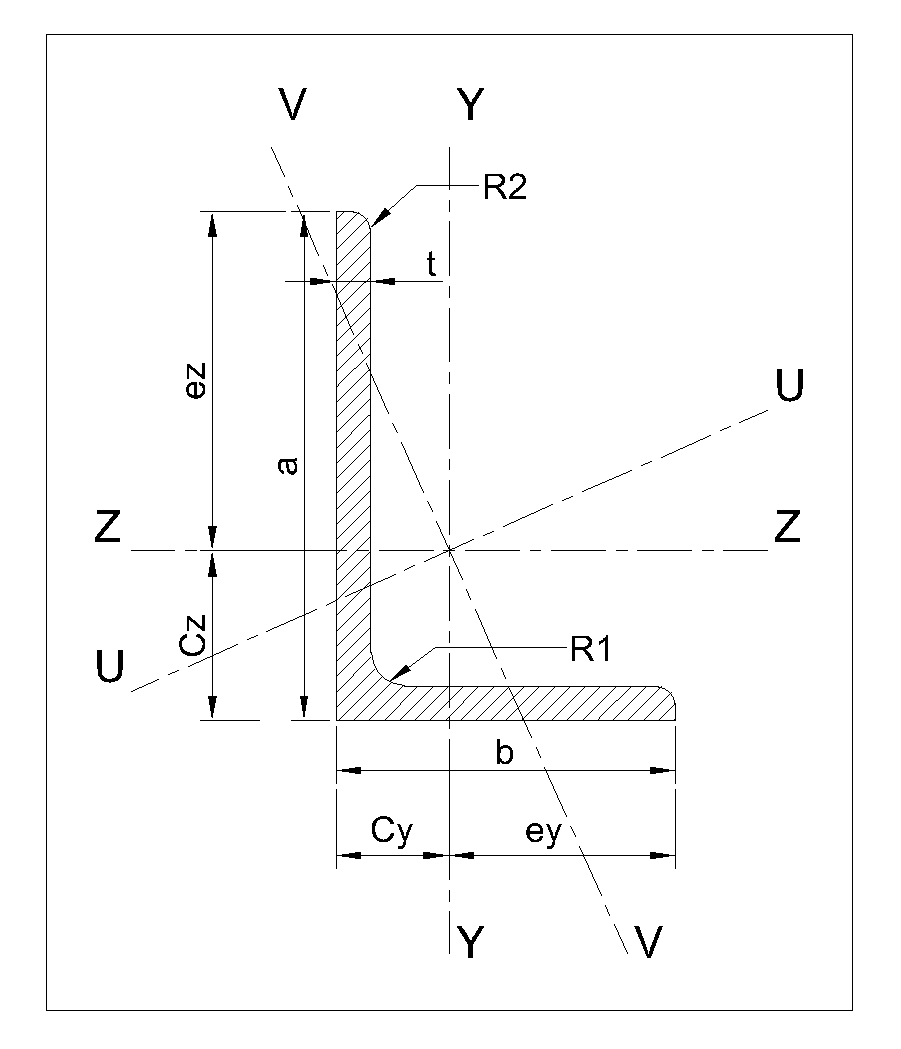
\includegraphics[width=5cm,height=5cm]{E:/workspace/Osdag3/ResourceFiles/images/Unequal.png}}&\multicolumn{2}{|c|}{Section Size*}&\multicolumn{2}{|c|}{('100 75 X 12', 'Angles')}\\%
\cline{2%
-%
5}%
&\multicolumn{2}{|c|}{Material *}&\multicolumn{2}{|c|}{E 250 (Fe 410 W)A}\\%
\cline{2%
-%
5}%
&\multicolumn{2}{|c|}{Ultimate strength, fu (MPa)}&\multicolumn{2}{|c|}{410}\\%
\cline{2%
-%
5}%
&\multicolumn{2}{|c|}{Yield Strength , fy (MPa)}&\multicolumn{2}{|c|}{230}\\%
\cline{2%
-%
5}%
&Mass&15.4&Iu(mm4)&2112000.0\\%
\cline{2%
-%
5}%
&Area(mm2) {-} A&1960.0&Iv(mm4)&661000.0\\%
\cline{2%
-%
5}%
&A(mm)&100.0&rz(mm)&30.9\\%
\cline{2%
-%
5}%
&B(mm)&75.0&ry(mm)&21.4\\%
\cline{2%
-%
5}%
&t(mm)&12.0&ru(mm)&32.8\\%
\cline{2%
-%
5}%
&R1(mm)&8.5&rv(mm)&18.4\\%
\cline{2%
-%
5}%
&R2(mm)&0.0&Zz(mm3)&27800.0\\%
\cline{2%
-%
5}%
&Cy(mm)&20.6&Zy(mm3)&16600.0\\%
\cline{2%
-%
5}%
&Cz(mm)&32.7&Zpz(mm3)&50900.0\\%
\cline{2%
-%
5}%
&Iz(mm4)&1870000.0&Zpy(mm3)&16600.0\\%
\cline{2%
-%
5}%
&Iy(mm4)&900000.0&r(mm3)&18.4\\%
\cline{2%
-%
5}%
\hline%
\multicolumn{5}{|c|}{\textbf{Bolt Details}}\\%
\hline%
\hline%
\multicolumn{3}{|c|}{Diameter (mm)*}&\multicolumn{2}{|c|}{{[}12.0, 16.0, 20.0, 24.0, 30.0, 36.0{]}}\\%
\hline%
\hline%
\multicolumn{3}{|c|}{Grade *}&\multicolumn{2}{|c|}{{[}3.6, 4.6, 4.8, 5.6, 5.8, 6.8, 8.8, 9.8, 10.9, 12.9{]}}\\%
\hline%
\hline%
\multicolumn{3}{|c|}{Type *}&\multicolumn{2}{|c|}{Bearing Bolt}\\%
\hline%
\hline%
\multicolumn{3}{|c|}{Bolt hole type}&\multicolumn{2}{|c|}{Standard}\\%
\hline%
\hline%
\multicolumn{3}{|c|}{Bolt Ultimate Strength (N/mm2)}&\multicolumn{2}{|c|}{1000.0}\\%
\hline%
\hline%
\multicolumn{3}{|c|}{Bolt Yield Strength (N/mm2)}&\multicolumn{2}{|c|}{900.0}\\%
\hline%
\hline%
\multicolumn{3}{|c|}{Slip factor (µ\_f)}&\multicolumn{2}{|c|}{0.3}\\%
\hline%
\hline%
\multicolumn{3}{|c|}{Type of edges}&\multicolumn{2}{|c|}{a {-} Sheared or hand flame cut}\\%
\hline%
\hline%
\multicolumn{3}{|c|}{Gap between beam and <br>support (mm)}&\multicolumn{2}{|c|}{0.0}\\%
\hline%
\hline%
\multicolumn{3}{|c|}{Are the members exposed to <br>corrosive influences}&\multicolumn{2}{|c|}{False}\\%
\hline%
\hline%
\multicolumn{5}{|c|}{\textbf{Safety Factors {-} IS 800:2007 Table 5 (Clause 5.4.1) }}\\%
\hline%
\hline%
\multicolumn{3}{|c|}{Governed by Yielding}&\multicolumn{2}{|c|}{$\begin{aligned}\gamma_{m0}&=1.1\end{aligned}$}\\%
\hline%
\hline%
\multicolumn{3}{|c|}{Governed by Ultimate Stress}&\multicolumn{2}{|c|}{$\begin{aligned}\gamma_{m1}&=1.25\end{aligned}$}\\%
\hline%
\hline%
\multicolumn{3}{|c|}{Connection Bolts {-} Bearing Type}&\multicolumn{2}{|c|}{$\begin{aligned}\gamma_{mb}&=1.25\end{aligned}$}\\%
\hline%
\end{longtable}

%
\Needspace{10\baselineskip}%
\newpage%
\section{Design Checks}%
\label{sec:DesignChecks}%
\subsection{Member Checks}%
\label{subsec:MemberChecks}%
\renewcommand{\arraystretch}{1.2}%
\begin{longtable}{|p{2.5cm}|p{5cm}|p{7.5cm}|p{1cm}|}%
\hline%
\rowcolor{OsdagGreen}%
Check&Required&Provided&Remarks\\%
\hline%
\endhead%
\hline%
Tension Yielding Capacity (kN)&&$\begin{aligned}T_{dg}~or~A_c&= \frac{1 * A_g ~ f_y}{\gamma_{m0}}\\ &= \frac{1*1960.0*230}{1.1}\\ &= 409.82\end{aligned}$&\\%
\hline%
Tension Rupture Capacity (kN)&&$\begin{aligned}\beta &= 1.4 - 0.076*\frac{w}{t}*\frac{f_{y}}{0.9*f_{u}}*\frac{b_s}{L_c}\\ &\leq\frac{0.9*f_{u}*\gamma_{m0}}{f_{y}*\gamma_{m1}} \geq 0.7 \\ &= 1.4 - 0.076*\frac{75.0}{12.0}*\frac{230}{0.9*410}*\frac{123.25}{225 }\\ &\leq\frac{0.9* 410*1.1}{230*1.25} \geq 0.7 \\ &= 1.24\\ T_{dn} &= 1*(\frac{0.9*A_{nc}*f_{u}}{\gamma_{m1}} + \frac{\beta * A_{go} * f_{y}}{\gamma_{m0}})\\ &= 1*(\frac{0.9* 840.0*410}{1.25} + \frac{1.24*900.0*230}{1.1})\\ &= 481.31\end{aligned}$&\\%
\hline%
Block Shear Capacity (kN)&&$\begin{aligned}T_{db1} &= \frac{A_{vg} f_{y}}{\sqrt{3} \gamma_{m0}} + \frac{0.9 A_{tn} f_{u}}{\gamma_{m1}}\\ T_{db2} &= \frac{0.9*A_{vn} f_{u}}{\sqrt{3} \gamma_{m1}} + \frac{A_{tg} f_{y}}{\gamma_{m0}}\\ T_{db} &= min(T_{db1}, T_{db2})= 429.01\end{aligned}$&\\%
\hline%
Tension Capacity (kN)&400.0&$\begin{aligned} T_d &= Min(T_{dg},T_{dn},T_{db})\\ &= Min(409.82,481.31,429.01)\\ &=409.82\end{aligned}$&Pass\\%
\hline%
Slenderness&$\begin{aligned}\frac{K * L}{r} &\leq 400\end{aligned}$&$\begin{aligned}\frac{K * L}{r} &= \frac{1*2000.0}{18.4}\\ &= 108.7\end{aligned}$&\\%
\hline%
Utilization Ratio&$\begin{aligned} Utilization~Ratio &\leq 1 \end{aligned}$&$\begin{aligned} Utilization~Ratio &= \frac{F}{Td}&=\frac{400.0}{409.82}\\ &= 0.98\end{aligned}$&\\%
\hline%
Axial Load Considered (kN)&$\begin{aligned} Ac_{min} &= 0.3 * A_c\\ &= 0.3 *409.82\\ &=122.95\\ Ac_{max} &=409.82\\$&$\begin{aligned} A_c &=400000.0 \end{aligned}$&\\%
\hline%
\end{longtable}

%
\newpage%
\subsection{Bolt Checks}%
\label{subsec:BoltChecks}%
\renewcommand{\arraystretch}{1.2}%
\begin{longtable}{|p{2.5cm}|p{5.5cm}|p{7cm}|p{1cm}|}%
\hline%
\rowcolor{OsdagGreen}%
Check&Required&Provided&Remarks\\%
\hline%
\endhead%
\hline%
Diameter (mm)&Bolt Quantity Optimisation&$\begin{aligned} d &=16.0 \end{aligned}$&\\%
\hline%
Grade&Bolt Grade Optimisation&10.9&\\%
\hline%
Hole Diameter (mm)& &$\begin{aligned} d_0 &=18.0 \end{aligned}$&\\%
\hline%
Nominal Stress Area (mm2)& &$\begin{aligned} A_{nb} &=157 \end{aligned}$&\\%
\hline%
Shear Capacity (kN)&&$\begin{aligned}V_{dsb} &= \frac{f_ub ~n_n~ A_{nb}}{\sqrt{3} ~\gamma_{mb}}\\ &= \frac{1000.0*1*157}{\sqrt{3}~*~1.25}\\ &= 72.52\end{aligned}$&\\%
\hline%
Bearing Capacity (kN)&&$\begin{aligned}V_{dpb} &= \frac{2.5~ k_b~ d~ t~ f_u}{\gamma_{mb}}\\ &= \frac{2.5~*0.58*16.0*12.0*410}{1.25}\\ &=91.32\end{aligned}$&\\%
\hline%
Capacity (kN)&&$\begin{aligned}V_{db} &= min~ (V_{dsb}, V_{dpb})\\ &= min~ (72.52,91.32)\\ &=72.52\end{aligned}$&\\%
\hline%
No of Bolts&$\begin{aligned}R_{u} &= \sqrt{V_u^2+A_u^2}\\ n_{trial} &= R_u/ V_{bolt}\\ R_{u} &= \frac{\sqrt{0.0^2+400.0^2}}{72.52}\\ &=6\end{aligned}$&$\begin{aligned} n &=6 \end{aligned}$&\\%
\hline%
No of Columns&&$\begin{aligned} n_c &=6 \end{aligned}$&\\%
\hline%
No of Rows&&$\begin{aligned} n_r &=1 \end{aligned}$&\\%
\hline%
Min. Pitch (mm)&$\begin{aligned}p/g_{min}&= 2.5 ~ d&\\ =&2.5*16.0&=40.0\end{aligned}$&45&Pass\\%
\hline%
Max. Pitch (mm)&$\begin{aligned}p/g_{max} &=\min(32~t,~300~mm)&\\ &=\min(32 *~12.0,~ 300 ~mm)\\&=300\end{aligned}$&45&Pass\\%
\hline%
Min. Gauge (mm)&$\begin{aligned}p/g_{min}&= 2.5 ~ d&\\ =&2.5*16.0&=40.0\end{aligned}$&0&N/A\\%
\hline%
Max. Gauge (mm)&$\begin{aligned}p/g_{max} &=\min(32~t,~300~mm)&\\ &=\min(32 *~12.0,~ 300 ~mm)\\&=300\end{aligned}$&0&N/A\\%
\hline%
Min. End Distance (mm)&$\begin{aligned}e/e`_{min} &=[1.5~or~ 1.7] * d_0\\ &=1.7*18.0=30.6 \end{aligned}$&35&Pass\\%
\hline%
Max. End Distance (mm)&$\begin{aligned}e/e`_{max} &= 12~ t~ \varepsilon&\\ \varepsilon &= \sqrt{\frac{250}{f_y}}\\ e/e`_{max}&=12 ~*20.0*\sqrt{\frac{250}{230}}\\ &=249.6\\ \end{aligned}$&35&Pass\\%
\hline%
Min. Edge Distance (mm)&$\begin{aligned}e/e`_{min} &=[1.5~or~ 1.7] * d_0\\ &=1.7*18.0=30.6 \end{aligned}$&39.75&Pass\\%
\hline%
Max. Edge Distance (mm)&$\begin{aligned}e/e`_{max} &= 12~ t~ \varepsilon&\\ \varepsilon &= \sqrt{\frac{250}{f_y}}\\ e/e`_{max}&=12 ~*20.0*\sqrt{\frac{250}{230}}\\ &=249.6\\ \end{aligned}$&39.75&Pass\\%
\hline%
Bolt Capacity post Long Joint (kN)&$\begin{aligned} &if~l\geq 15 * d~then~V_{rd} = \beta_{ij} * V_{db} \\ & if~l < 15 * d~then~V_{rd} = V_{db} \\ & where,\\ & l = ((nc~or~nr) - 1) * (p~or~g) \\ & \beta_{ij} = 1.075 - l/(200 * d) \\ & but~0.75\leq\beta_{ij}\leq1.0 \end{aligned}$&$\begin{aligned} l&= ((nc~or~nr) - 1) * (p~or~g) \\  &= (6 - 1) * 45=225\\  &= (1 - 1) * 0=0\\  l&= 225\\ & 15 * d = 15 * 16.0 = 240.0 \\ & since,~l < 15 * d~then~V_{rd} = V_{db} \\ & V_{rd} = 72.52 \end{aligned}$&\\%
\hline%
Capacity (kN)&66.67&72.52&Pass\\%
\hline%
\end{longtable}

%
\newpage%
\subsection{Gusset Plate Checks}%
\label{subsec:GussetPlateChecks}%
\renewcommand{\arraystretch}{1.2}%
\begin{longtable}{|p{2.5cm}|p{5cm}|p{7.5cm}|p{1cm}|}%
\hline%
\rowcolor{OsdagGreen}%
Check&Required&Provided&Remarks\\%
\hline%
\endhead%
\hline%
Height (mm)&&$\begin{aligned} H &= 1* Depth + clearance \\ &=(1*100.0)+30.0\\ &= 130.0\end{aligned}$&\\%
\hline%
Length (mm)&&$\begin{aligned} L &= (nc -1) * p + 2 * e\\ &= (6-1) *45+ (2 *35)\\ &= 295\end{aligned}$&\\%
\hline%
Thickness (mm)&&$\begin{aligned} t_p &=20.0 \end{aligned}$&\\%
\hline%
Tension Yielding Capacity (kN)&&$\begin{aligned} T_{dg} &= \frac{Depth*t_p*f_y}{\gamma_{mo}}\\ &=\frac{100.0*20.0*230}{1.1}\\ &=418.18\end{aligned}$&\\%
\hline%
Tension Rupture Capacity (kN)&&$\begin{aligned} T_{dn} &= \frac{0.9*A_{n}*f_u}{\gamma_{m1}}\\ &=\frac{0.9*(100.0-1*18.0)*20.0*410}{1.25}\\ &=484.13\end{aligned}$&\\%
\hline%
Block Shear Capacity (kN)&&$\begin{aligned}T_{db1} &= \frac{A_{vg} f_{y}}{\sqrt{3} \gamma_{m0}} + \frac{0.9 A_{tn} f_{u}}{\gamma_{m1}}\\ T_{db2} &= \frac{0.9*A_{vn} f_{u}}{\sqrt{3} \gamma_{m1}} + \frac{A_{tg} f_{y}}{\gamma_{m0}}\\ T_{db} &= min(T_{db1}, T_{db2})= 715.02\end{aligned}$&\\%
\hline%
Tension Capacity (kN)&400.0&$\begin{aligned} T_d &= Min(T_{dg},T_{dn},T_{db})\\ &= Min(418.18,484.13,715.02)\\ &=418.18\end{aligned}$&Pass\\%
\hline%
\end{longtable}

%
\Needspace{10\baselineskip}%
\newpage%
\section{3D View}%
\label{sec:3DView}%


\begin{figure}[h!]%
\centering%
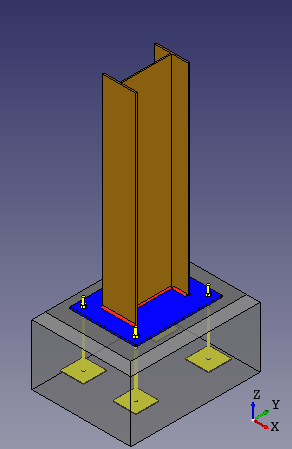
\includegraphics[width=\linewidth]{E:/workspace/Osdag3/ResourceFiles/images/3d.png}%
\caption{3D View}%
\end{figure}

%
\end{document}